\subsection{Analisis de sensibilidades}

Se calcularon las sensibilidades de cada FT para $\omega_p$ y $bw_p$ con respecto a cada componente. Para ello se hizo uso de PYTHON y las propiedades desarrolladas en el Daryanani para las sensibilidades.

\begin{figure}[H]
    \centering
    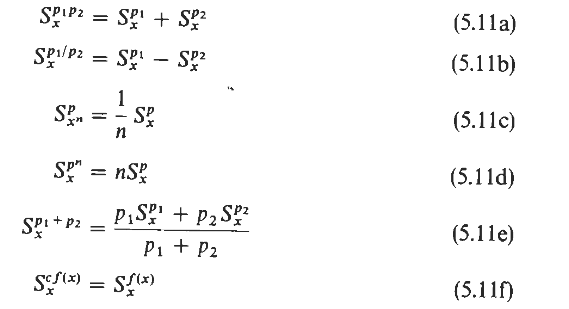
\includegraphics[scale=.5]{Secciones/Circ1/img/daryanani149.png}
    \caption{Propiedades para la sensibilidad (Daryanani pag. 149).}
    \label{prop}
\end{figure}

Luego se comprobaron los resultados obtenidos con las identidades de verificacion que nos da el Daryanani.

\begin{figure}[H]
    \centering
    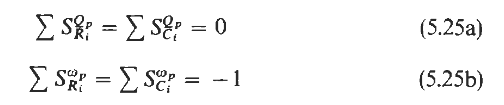
\includegraphics[scale=.5]{Secciones/Circ1/img/daryanani155.png}
    \caption{Identidades de verificacion (Daryanani pag. 155).}
    \label{prop}
\end{figure}

Y finalmente se reemplazaron los valores de componentes y obtuvieron los valores de sensibilidad para cada circuito.

\subsubsection{Realimentacion positiva (Sallen-Key)}

\noindent $>>$ \texttt{Recordando la topologia analizada y la FT \eqref{posFT} obtenida:}

\begin{figure}[H]
    \centering
    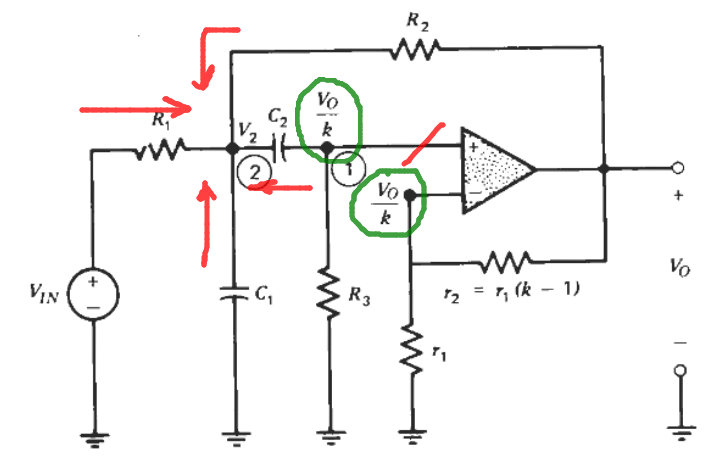
\includegraphics[scale=.5]{Secciones/Circ1/img/sallenKeyBP.png}
    \caption{Topologia de realimentacion positiva (Sallen-Key BP).}
    \label{c1}
\end{figure}

\noindent $>>$ \texttt{Se identifican por inpeccion los parametros:}

\begin{align*}
    \omega_p^{2} &= \frac{1}{R_{1} C_{1} R_{3} C_{2}} + \frac{1}{R_{2} C_{2} R_{3} C_{1}}
    = \omega_{1} \omega_{32} + \omega_{2} \omega_{31}  \\ 
    \frac{\omega_{p}}{Q_{p}} &= bw_p 
    = \frac{1}{R_{2} C_{1}} (1-k) + \frac{1}{R_{1} C_{1}} + \frac{1}{R_{3} C_{1}} + \frac{1}{R_{3} C_{2}} 
    = \omega_{21} (1-k) + \omega_{1} + \omega_{31} + \omega_{32}
\end{align*}

$$
\text{Donde por simplicidad se define (con 1 o 2 sub-indices) }
\omega=\begin{cases}
            \omega_{ij}=\frac{1}{R_{i} C_{j}}, \quad si \quad i\neq j \\
            \omega_{i}=\frac{1}{R_{i} C_{i}}, \quad si\quad i=j
        \end{cases}
$$

De esta forma se identifico que por ejemplo $\omega_{p}^{2}$ esta compuesto por una suma de productos de parametros.

Con esto en mente se empezaron a aplicar las propiedades para la suma y producto de sensibilidades.

\begin{gather*}
    \texttt{Como es una suma:} \\\\
    S^{\omega_{p}^{2}}_{x}=\frac{\omega_1 \omega_{32} S^{\omega_1 * \omega_{32}}_{x} + \omega_2 \omega_{31} S^{\omega_2 * \omega_{31}}_{x}}{\omega_1 \omega_{32} + \omega_2 \omega_{31}} \\\\
    \texttt{Desarrollando los productos:} \\\\
    S^{\omega_1 * \omega_{32}}_{x} = S^{\omega_1}_{x} + S^{\omega_{32}}_{x} \\ 
    S^{\omega_2 * \omega_{31}}_{x} = S^{\omega_2}_{x} + S^{\omega_{31}}_{x} \\\\
    S^{\omega_{p}^{2}}_{x} = \frac{\omega_1 \omega_{32} (S^{\omega_1}_{x} + S^{\omega_{32}}_{x}) + \omega_2 \omega_{31} (S^{\omega_2}_{x} + S^{\omega_{31}}_{x})}{\omega_1 \omega_{32} + \omega_2 \omega_{31}} \\\\
    \texttt{Y aplicando la propiedad para la potencia:} \\\\
    S^{\omega_{p}^{2}}_{x} = 2 S^{\omega_{p}}_{x}
\end{gather*}

\noindent $>>$ \texttt{Donde x representa cualquier componente del circuito, por ejemplo para la sensibilidad de los parametros respecto de R1 se tiene:}

\begin{align*}
    S^{\omega_1}_{R1} = -1, \quad
    S^{\omega_{32}}_{R1} = 0, \quad
    S^{\omega_{2}}_{R1} = 0, \quad
    S^{\omega_{31}}_{R1} = 0
\end{align*}

\noindent $>>$ \texttt{Reemplazando para el parametro que nos interesa:}

\begin{equation*}
    S^{\omega_{p}}_{R1} = - \frac{1}{2} \frac{R_{2}}{R_{1} + R_{2}}
\end{equation*} \\

Siguiendo este procedimiento se obtuvieron las sensibilidades de los parametros de interes respecto de todos los componentes del circuito. \\
Para acelerar el proceso se trabajo con ecuaciones simbolicas en PYTHON.\\

Sensibilidades para $\omega_{p}$:

\begin{align*}
    S^{\omega_{p}}_{R1} &= - \frac{1}{2} \frac{R_{2}}{R_{1} + R_{2}}  &
    S^{\omega_{p}}_{C1} &= - \frac{1}{2} \\
    S^{\omega_{p}}_{R2} &= - \frac{1}{2} \frac{R_{1}}{R_{1} + R_{2}}  &
    S^{\omega_{p}}_{C2} &= - \frac{1}{2} \\
    S^{\omega_{p}}_{R3} &= - \frac{1}{2}
\end{align*}

Sensibilidades para $bw_{p}$:

\begin{align*}
    S^{bw_p}_{R1} &= - \frac{1}{C_{1} R_{1}} \frac{1}{bw_p}  &
    S^{bw_p}_{C1} &= - \frac{R_{1} R_{2} + R_{1} R_{3}  (1 - k) + R_{2} R_{3}}{C_{1} R_{1} R_{2} R_{3}} \frac{1}{bw_p} \\
    S^{bw_p}_{R2} &= - \frac{1-k}{C_{1} R_{2}} \frac{1}{bw_p}  &
    S^{bw_p}_{C2} &= - \frac{1}{C_{2} R_{3}} \frac{1}{bw_p} \\
    S^{bw_p}_{R3} &= - \frac{C_{1} + C_{2}}{C_{1} C_{2} R_{3}} \frac{1}{bw_p}
\end{align*}

Tambien se comprobaron mediante PYTHON las igualdades de verificacion de $S^{\omega_{p}}_{x}$ y $S^{Q_p}_{x}$; obteniendo esta ultima aplicando la propiedad de cociente de sensibilidades para $S^{bw_p}_{x}$ y despejando $S^{Q_p}_{x}$:

\begin{align*}
    \sum_{i=1}^{3} S^{\omega_p}_{R_i} &= \sum_{i=1}^{2} S^{\omega_p}_{C_i} = -1 \\
    \sum_{i=1}^{3} S^{Q_p}_{R_i} &= \sum_{i=1}^{2} S^{Q_p}_{C_i} = 0
\end{align*}

Finalmente se reemplazaron los valores de los componentes por los utilizados en la implementacion del circuito, para obtener las sensibilidades de la primer etapa con topologia de realimentacion positiva. \\

Como: $C_{1}=100 nF, \quad C_{2}=100 nF, \quad R=1738 \Omega, \quad k=3.44$ 
    
\begin{align}
    &\mathbf{S^{\omega_{p}}_{R1} = S^{\omega_{p}}_{R2} = -0.25, \quad S^{\omega_{p}}_{R3} = -0.5} \\
    &\mathbf{S^{\omega_{p}}_{C1} = S^{\omega_{p}}_{C2} = -0.5}
\end{align}

\begin{align}
    &\mathbf{S^{bw_{p}}_{R1} = -1.81, \quad S^{bw_{p}}_{R2} = 4.41, \quad S^{bw_{p}}_{R3} = -3.61} \\
    &\mathbf{S^{bw_{p}}_{C1} = 0.79, \quad S^{bw_{p}}_{C2} = -1.81}
\end{align}

% -----------------------

\subsubsection{Realimentacion negativa}

\noindent $>>$ \texttt{Recordando la topologia analizada y la FT \eqref{negFT}}

\begin{figure}[H]
    \centering
    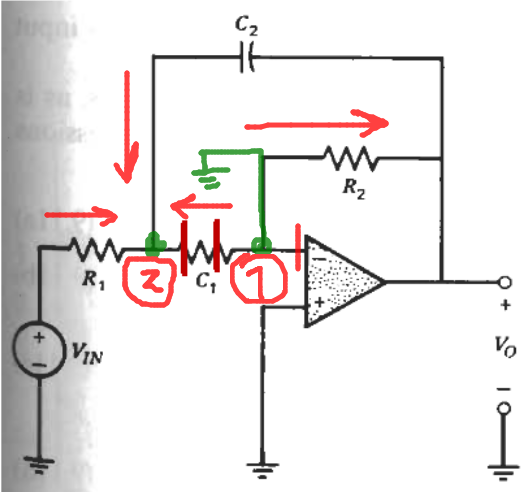
\includegraphics[scale=.5]{Secciones/Circ1/img/negBiquadBP.png}
    \caption{Topologia de realimentacion negativa.}
    \label{c1}
\end{figure}

\noindent $>>$ \texttt{Por inpeccion indentificamos los parametros:}

\begin{align*}
    \omega_p^{2} &= \frac{1}{R_{1} C_{1} R_{2} C_{2}}
    = \omega_{1} \omega_{2} \\ 
    \frac{\omega_{p}}{Q_{p}} &= bw_p 
    = \frac{1}{R_{2} C_{2}} + \frac{1}{R_{2} C_{1}}
    = \omega_{2} + \omega_{21}
\end{align*}

$$
\text{Donde por simplicidad se define (con 1 o 2 sub-indices) }
\omega=\begin{cases}
            \omega_{ij}=\frac{1}{R_{i} C_{j}}, \quad si \quad i\neq j \\
            \omega_{i}=\frac{1}{R_{i} C_{i}}, \quad si\quad i=j
        \end{cases}
$$

Se aplicaron las propiedades para las sensibilidades y se siguio el mismo procedimiento para obtener las sensibilidades de los parametros de interes respecto de todos los componentes del circuito. \\

Sensibilidades para $\omega_{p}$:

\begin{align*}
    S^{\omega_{p}}_{R1} &= - 0.5  &
    S^{\omega_{p}}_{C1} &= - 0.5 \\
    S^{\omega_{p}}_{R2} &= - 0.5  &
    S^{\omega_{p}}_{C2} &= - 0.5 \\
\end{align*}

Sensibilidades para $bw_{p}$:

\begin{align*}
    S^{bw_p}_{R1} &= 0  &
    S^{bw_p}_{C1} &= - \frac{C_{2}}{C_{1} + C_{2}} \\
    S^{bw_p}_{R2} &= - 1  &
    S^{bw_p}_{C2} &= - \frac{C_{1}}{C_{1} + C_{2}}
\end{align*}

\noindent $>>$ \texttt{Se comprobaron mediante PYTHON las igualdades de verificacion para validar las expresiones encontradas:}

\begin{align*}
    \sum_{i=1}^{2} S^{\omega_p}_{R_i} &= \sum_{i=1}^{2} S^{\omega_p}_{C_i} = -1 \\
    \sum_{i=1}^{2} S^{Q_p}_{R_i} &= \sum_{i=1}^{2} S^{Q_p}_{C_i} = 0
\end{align*}

Finalmente se reemplazaron los valores de los componentes por los utilizados en la implementacion del circuito, para obtener las sensibilidades de la segunda etapa con topologia de realimentacion negativa. \\

Como: $C_{1}=100 nF, \quad C_{2}=100 nF, \quad R1=410 \Omega, \quad R2=10560 \Omega$ 
    
\begin{align}
    &\mathbf{S^{\omega_{p}}_{R1} = S^{\omega_{p}}_{R2} = -0.5} \\
    &\mathbf{S^{\omega_{p}}_{C1} = S^{\omega_{p}}_{C2} = -0.5}
\end{align}

\begin{align}
    &\mathbf{S^{bw_{p}}_{R1} = 0, \quad S^{bw_{p}}_{R2} = -1} \\
    &\mathbf{S^{bw_{p}}_{C1} = S^{bw_{p}}_{C2} = -0.5}
\end{align}